\documentclass{beamer}

\setbeamertemplate{caption}{\raggedright\insertcaption\par}

\mode<presentation>
{
  \usetheme{CambridgeUS}

  \setbeamercovered{transparent}
}


\definecolor{Or}{RGB}{255,153,000}
\definecolor{Indigo}{RGB}{72,61,139}
\definecolor{Magenta}{RGB}{139,0,139}

\setbeamercolor{normal text}{fg=black,bg=white}
\setbeamercolor{alerted text}{fg=Indigo}
\setbeamercolor{example text}{fg=Indigo}

%\setbeamercolor{background canvas}{fg=myforeground, bg=white}
%\setbeamercolor{background}{fg=myforeground, bg=mybackground}
%
%\setbeamercolor{palette primary}{fg=black, bg=gray!30!white}
%\setbeamercolor{palette secondary}{fg=black, bg=gray!20!white}
%\setbeamercolor{palette tertiary}{fg=black, bg=gold}



\setbeamercolor{palette tertiary}{fg=black, bg=Indigo}
\setbeamercolor{frametitle}{fg=Indigo}
\setbeamercolor{title}{fg=Indigo}
\setbeamercolor{footline}{fg=Indigo, bg=Indigo}
\setbeamercolor{author in head/foot}{fg=black}
\setbeamercolor{date in head/foot}{fg=black}
\setbeamercolor{title in head/foot}{fg=black}

\definecolor{Highlight}{RGB}{139,0,139}
\newcommand{\HL}[1]{{\color{Highlight}#1}}

\usefonttheme{professionalfonts}
\beamertemplatenavigationsymbolsempty

\usepackage[english]{babel}
\usepackage{color}
\usepackage{amsfonts}
\usepackage{amssymb}
\usepackage{epsfig}
\usepackage{amsmath}
\usepackage{txfonts}
\usepackage{relsize}

%\usepackage{bbold}
\usepackage{dsfont}
\usepackage{bbm}

\usepackage[latin1]{inputenc}

\newcommand{\id}{\mathbbm{1}}
\newcommand{\HH}{\mathcal{H}}
\newcommand{\CC}{\mathbb{C}}
\newcommand{\BB}{\mathcal{B}}
\newcommand{\dd}{\mathrm{d}}
\newcommand{\UU}{\mathcal{U}}
\newcommand{\ZZ}{\mathbb{Z}}
\newcommand{\tr}{\mathrm{tr}}
\newcommand{\Tr}{\mathrm{Tr}}
\renewcommand{\AA}{\mathcal{A}}



\newcommand{\mean}[1]{\langle #1 \rangle}
\newcommand{\cumul}[1]{\langle\!\langle #1 \rangle\!\rangle}

\DeclareRobustCommand{\augiefamily}{%
  \fontfamily{augie}\fontseries{m}\fontshape{n}\selectfont}
\DeclareTextFontCommand{\textaugie}{\augiefamily}

\usepackage{physics}

\setlength{\parskip}{0.1cm}

\title[SPT classification]%\hspace{1cm} \insertframenumber/\inserttotalframenumber]
{SPT classification:\\from matrix product states to recent proofs}

\author[Tijl]
{Tijl Jappens \\
 \scriptsize KU Leuven}


\institute[]{
instituut voor theorethische fysica KU Leuven
}


\date{\today}

\setbeamertemplate{itemize items}{\color{black}$\triangleright$}
\setbeamertemplate{enumerate items}{\color{black}\insertenumlabel.}

\usepackage[T1]{fontenc}
\DeclareRobustCommand{\augiefamily}{%
  \fontfamily{augie}\fontseries{m}\fontshape{n}\selectfont}
\DeclareTextFontCommand{\textaugie}{\augiefamily}

\begin{document}

%%%%%%%%%% Removes the frame number from the title page %%%%%%%%%%
\bgroup
\makeatletter
\setbeamertemplate{footline}
{
  \leavevmode%
  \hbox{%
  \begin{beamercolorbox}[wd=.333333\paperwidth,ht=2.25ex,dp=1ex,center]{author in head/foot}%
 %   \usebeamerfont{author in head/foot}\insertshortauthor\expandafter\beamer@ifempty\expandafter{\beamer@shortinstitute}{}{~~(\insertshortinstitute)}
  \end{beamercolorbox}%
  \begin{beamercolorbox}[wd=.333333\paperwidth,ht=2.25ex,dp=1ex,center]{title in head/foot}%
%    \usebeamerfont{title in head/foot}\insertshorttitle
  \end{beamercolorbox}%
  \begin{beamercolorbox}[wd=.333333\paperwidth,ht=2.25ex,dp=1ex,right]{date in head/foot}%
%    \usebeamerfont{date in head/foot}\insertshortdate{}\hspace*{2em}
%    \insertframenumber{} / \inserttotalframenumber\hspace*{2ex} 
  \end{beamercolorbox}}%
  \vskip0pt%
}
\makeatother
\begin{frame}
\titlepage
\end{frame}
\egroup

\setcounter{framenumber}{0}

\begin{frame}{Matrix product state}
\begin{columns}
\begin{column}{0.5\textwidth}
Hilbert space
\[\HH := \bigotimes_{n=0}^{L}\CC^{d}.\]
\end{column}
\begin{column}{0.5\textwidth}
\begin{itemize}
\item $L$ is chain length.
\item $d$ is on site dimension.
\end{itemize}
\end{column}
\end{columns}
\pause
\begin{block}{Definition: Matrix product state (MPS)}
$\ket{\psi}\in\HH$ is a MPS (with periodic boundary) if $\exists D<<L:\forall n\in\{0,..,L\}:\forall i\in\{1,..,d\}:\exists A^i_n\in\BB(\CC^D):$
\begin{equation}
\ket{\psi}=\sum_{i_1,..,i_L}\Tr(A^{i_1}_1\cdots A^{i_L}_L)\ket{i_1,\cdots i_L}.
\end{equation}
\end{block}
\pause
\begin{itemize}
\item D is called bond dimension.
\end{itemize}
\end{frame}

\begin{frame}{On site group action}
Let $G$ be a compact group. Take
\begin{align}
U(g)&\in\textrm{Hom}(G,U(\CC^d))&\tilde U(g)&:= \bigotimes_{n=0}^L U(g).
\end{align}
\pause
\begin{block}{Definition}
We say that an MPS $\ket{\psi}$ is SPT if $\exists \tilde{\alpha}\in\textrm{Hom}(G,U(1)):$
\[\tilde{U}(g)\ket{\psi}=\tilde{\alpha}(g)\ket{\psi}.\]
\end{block}
\end{frame}

\begin{frame}{On site group action on MPS}
\begin{block}{Lemma:}
Let $\ket{\psi}$ be an SPT then $\forall n\in\{0,L\}:$ $\exists R_n:G\rightarrow U(\CC^D)$ and $\alpha_n:G\rightarrow U(1)$ such that
\begin{equation}
\sum_{j=0}^{d}U(g)_{ij}A^j_n=\alpha_n(g) R_n(g)^\dagger A^i_n R_{n+1}(g)
\end{equation}
for all $g\in G.$
\end{block}
\pause
We can chose $\alpha_n$ to be a $U(1)$ representation
\[\alpha_n\in\textrm{Hom}(G,U(1))\]
\pause
and we can chose $R_n$ to be such that there exist $C_n:G^2\rightarrow U(1)$ such that
\[R_n(h)R_n(g)=C_n(g,h) R_n(gh).\]
\end{frame}

\begin{frame}{Properties of $C_n$}
Since $U(gh)^\dagger U(g)U(h)=\id$ we need
\begin{equation}
A_n^i=R_n(h)^\dagger R_n(g)^\dagger R_{n}(gh) A^i_n R_{n+1}(gh)^\dagger R_{n+1}(g) R_{n+1}(h)
\end{equation}
and therefore $C_n(g,h)=C_{n+1}(g,h)$. From now on:
\[C_1(g,h)=\cdots=C_L(g,h)=C(g,h).\]
\pause
Because of associativity
\begin{align*}
(R_n(g)R_n(h))R_n(l)&=R_n(g)(R_n(h)R_n(l))\\
C(g,h)C(gh,l)&=C(g,hl)C(h,l).
\end{align*}
C is a cochain (from group cohomology).
\end{frame}

\begin{frame}{Properties of $C_n$}
Note that for any $\beta:G\rightarrow U(1)$ changing the choice of $R_n:$
\[R_n(g)\rightarrow \beta(g)R_n(g)\]
is still consistent with everything up to now.
\pause
Define an equivalence class by saying that $(C_1)_{\sim}=(C_2)_{\sim}$ if there exists a $\beta:G\rightarrow U(1)$ such that:
\[C_1(g,h)=C_2(g,h)\beta(g)\beta(h)\overline{\beta(gh)}.\]
\pause
\begin{block}{Claim}
Let $C$ be the cochain defined up to now then $(C)_\sim$ is independent of the choice of $R_n$ and $\alpha_n$.
\end{block}
\pause
One dimensional SPT's are classified by an $H^2(G,U(1))-$valued index.
\end{frame}

\begin{frame}{Translation invariance}
A translation invariant MPS is of the form
\[\ket{\psi}=\sum_{i_1\cdots i_L}\textrm{Tr}(A^{i_1}\cdots A^{i_L})\ket{i_1,\cdots i_L}.\]
\pause
We still have $\exists \alpha\in\text{Hom}(G,U(1))$ and $R:G\rightarrow U(\CC^D)$ such that
 \[\sum_j U(g)_{ij}A^j=\alpha(g) R(g)^\dagger A^i R(g).\]
\pause
\begin{block}{Claim}
There exists an
\[H^2(G,U(1))\oplus \text{Hom}(G,U(1))=H^2(G,U(1))\oplus H^1(G,U(1))\]
valued index.
\end{block}
\end{frame}

\begin{frame}{Loops of SPT's}
Let
\begin{align}
H(\lambda)&= \sum_i H_i(\lambda)&U(\lambda)&= \mathcal{T}\exp(-i\int_0^\lambda \dd s H(s))
\end{align}
where each therm is $G-$invariant:
\[[H_i(\lambda),\tilde{U}(g)]=0.\]
\pause
Let $\ket{\psi}$ be a MPS SPT such that
\[U(1)\ket{\psi}\propto \ket{\psi}.\]
\end{frame}

\begin{frame}{Loops of SPT's: Making cuts}
\begin{columns}
\begin{column}{0.6\textwidth}
\onslide<1->{
\begin{align*}
H_R(\lambda)&=\sum_i H_i(\lambda)\chi(\textrm{supp}(H_i(\lambda))\subset R)\\
U_R(\lambda)&=\mathcal{T}\exp(-i \int_0^\lambda \dd s\: H_R(s) ).
\end{align*}
}
\onslide<2->{
Define
\[\ket{\psi_R}:= U_R(1)\ket{\psi}.\]
\begin{block}{Claim:}
\begin{itemize}
\item $\ket{\psi_R}$ is $G$-invariant and has same $\tilde{\alpha}(g)$.
\item $\ket{\psi_R}$ only differs from $\ket{\psi}$ around $B_1$ and $B_2$.
\end{itemize}
\end{block}
}
\end{column}
\onslide<1->{
\begin{column}{0.4\textwidth}
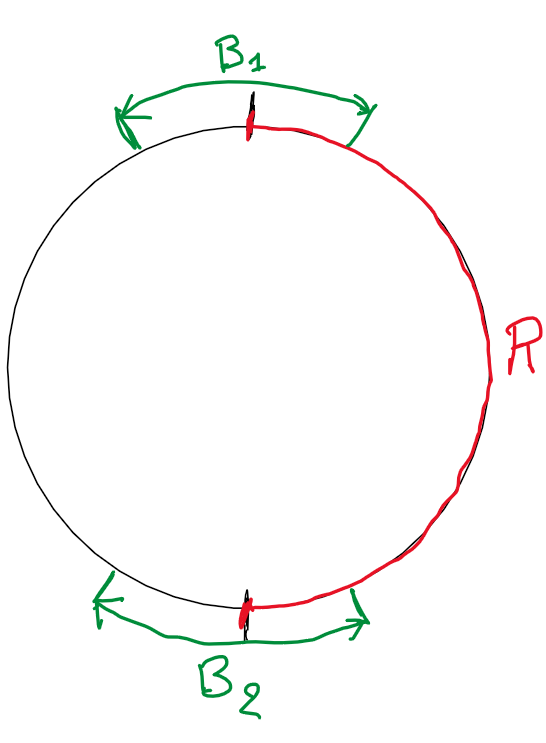
\includegraphics[width=\textwidth]{CircleRegions.png}
\end{column}
}
\end{columns}
\end{frame}

\begin{frame}{Loops of SPT's: Finite depth quantum cirquit}
A finite depth quantum cirquit (of depth 2) is of the form:
\begin{figure}
\center
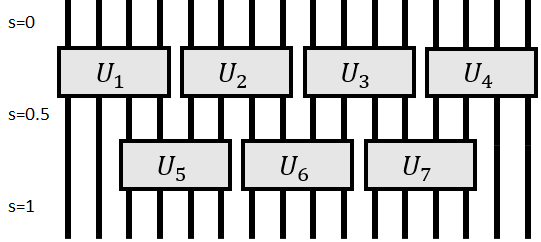
\includegraphics[width=0.8\textwidth]{FiniteDepthQuantumCirquit.png}
\end{figure}
\end{frame}

\begin{frame}{Loops of SPT's: Making previous statement precise}
\begin{columns}
\begin{column}{0.6\textwidth}
\begin{block}{Claim 1:}
Let $U_R(\lambda)$ be a finite depth quantum cirquit. $\exists\: B_1,B_2:\forall n\in B_1\cup B_2:\exists A'^i_n:$ such that $\ket{\psi_R}$ is $\ket{\psi}$ with the $A_n^i$ in $B_1\cup B_2$ replaced by $A'^i_n$.
\end{block}
\onslide<2->{
\begin{block}{Claim 2:}
Let $\ket{\psi_{1,R}}$ be the MPS that is $\ket{\psi}$ with the $A^i_n$ replaced by $A'^i_n$ in $B_1$ only then $\ket{\psi_{1,R}}$ is $G$-invariant as well.
\end{block}
}
\onslide<3->{
However $\tilde{\alpha}_1(g)/\tilde{\alpha}(g)$ need not be $1$. 
\[\tilde{\alpha}_1(g)/\tilde{\alpha}(g)\in H^1(G,U(1))\]
is called the charge pumping index.
}
\end{column}
\onslide<1->{
\begin{column}{0.4\textwidth}
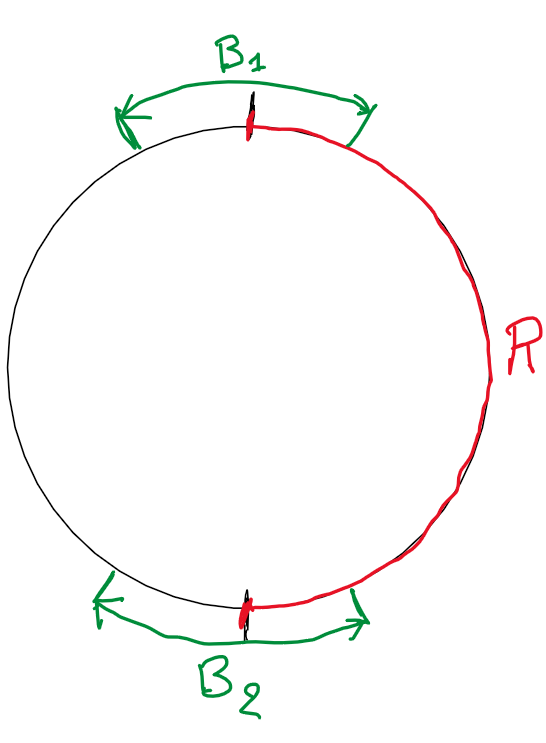
\includegraphics[width=\textwidth]{CircleRegions.png}
\end{column}
}
\end{columns}
\end{frame}

\begin{frame}{Quasi Local $C^*$ algebra}
Take
\begin{itemize}
\item $d$ the on site dimension.
\item $D$ the spatial dimension.
\item $\mathfrak{B}_{\ZZ^D}$ the local subsets of $\ZZ^D$.
\end{itemize}
\pause
We define the local $C^*$ algebra as follows: $\forall Z\in \mathfrak{B}_{\ZZ^D}\}:$
\begin{align*}
 \AA_Z&:=\bigotimes_{i\in Z}\left(\BB(\CC^d)\right)_i&\onslide<3->{\AA_{\text{loc}}&:=\{\AA_{Z} | Z\in \mathfrak{B}_{\ZZ^D}\}}.
\end{align*}
\onslide<4->{
\begin{block}{Definition: Quasi Local $C^*$ algebra}
We define $\AA$ as the norm closure of $\AA_{\text{loc}}$:
\[\AA:=\overline{\AA_{\text{loc}}}.\]
\end{block}}
\end{frame}

\begin{frame}{States and interactions}
$\omega:\AA\rightarrow \CC$ is a state if it is positive and linear.\\
\pause
\begin{itemize}
\item When will we say that two pure states are connected?
\pause
\item We won't define a topology only an equivalence class.
\end{itemize}
\pause
\begin{block}{Bounded Interaction}
An interaction is a map of the form
\[\Phi:\mathfrak{B}_{\ZZ^D}\rightarrow\textrm{Herm}(\AA_{\cdot}).\]
\pause
Additionally it is bounded if there exists a MDP function $f:\mathbb{N}^+\rightarrow \mathbb{R}^+$ decaying faster then any exponential such that
\[\norm{\Phi}_f:=\textrm{sup}_{j\in\ZZ^D}\sum_{S}\chi(j\in S)\frac{\norm{\Phi(S)}}{f(1+\textrm{diam}(S))}<\infty.\]
\end{block}
\end{frame}

\begin{frame}{Locally generated automorphism}
\begin{block}{Definition}
An automorphism $\alpha_\lambda:\AA\rightarrow \AA$ is locally generated if there exists a one parameter family of bounded interactions $\Phi_\lambda$ satisfying ($\forall a\in\AA$)
\[\frac{\dd}{\dd \lambda}\alpha_\lambda(a)=-i\alpha_\lambda\left(\sum_{S\in\mathfrak{B}_{\ZZ^D}}[\Phi_\lambda(S),a]\right).\]
\end{block}
\end{frame}

\end{document}


